%%%%%%%%%%%%%%%%%%%%%%%%%%%%%%%%%%%%%%%%%
% Stylish Article
% LaTeX Template
% Version 2.1 (1/10/15)
%
% This template has been downloaded from:
% http://www.LaTeXTemplates.com
%
% Original author:
% Mathias Legrand (legrand.mathias@gmail.com) 
% With extensive modifications by:
% Vel (vel@latextemplates.com)
%
% License:
% CC BY-NC-SA 3.0 (http://creativecommons.org/licenses/by-nc-sa/3.0/)
%
%%%%%%%%%%%%%%%%%%%%%%%%%%%%%%%%%%%%%%%%%

%----------------------------------------------------------------------------------------
%	PACKAGES AND OTHER DOCUMENT CONFIGURATIONS
%----------------------------------------------------------------------------------------

\documentclass[10pt]{SelfArx} % Document font size and equations flushed left

\usepackage[english]{babel} % Specify a different language here - english by default

\usepackage{lipsum} % Required to insert dummy text. To be removed otherwise

%----------------------------------------------------------------------------------------
%	COLUMNS
%----------------------------------------------------------------------------------------

%\setlength{\columnsep}{0.55cm} % Distance between the two columns of text
\setlength{\fboxrule}{0.75pt} % Width of the border around the abstract

%----------------------------------------------------------------------
%   BOX OF 'ANALYSIS' PART, MODIFIED FROM THE 'COROLLARY' ENVIORMENT
%----------------------------------------------------------------------

\newcounter{dummy} 
\numberwithin{dummy}{section}
\newtheorem{corollaryT}[dummy]{Corollary}
\usepackage[framemethod=default]{mdframed} % Required for creating the theorem, definition, exercise and corollary boxes 
% Corollary box
\newmdenv[skipabove=7pt,
skipbelow=7pt,
rightline=false,
leftline=true,
topline=false,
bottomline=false,
linecolor=gray,
backgroundcolor=black!5,
innerleftmargin=5pt,
innerrightmargin=5pt,
innertopmargin=5pt,
leftmargin=0.8cm,
rightmargin=0cm,
linewidth=4pt,
innerbottommargin=5pt]{cBox}
%\newenvironment{corollary}{\begin{cBox}\begin{corollaryT}}{\end{corollaryT}\end{cBox}}
\newenvironment{corollary}{\begin{cBox}\noindent{\bf\color{color1} 分析}}{\end{cBox}}





%----------------------------------------------------------------------------------------
%	COLORS
%----------------------------------------------------------------------------------------

\definecolor{color1}{RGB}{0,0,90} % Color of the article title and sections
\definecolor{color2}{RGB}{0,20,20} % Color of the boxes behind the abstract and headings

%----------------------------------------------------------------------------------------
%	HYPERLINKS
%----------------------------------------------------------------------------------------

\usepackage{hyperref} % Required for hyperlinks
\hypersetup{hidelinks,colorlinks,breaklinks=true,urlcolor=color2,citecolor=color1,linkcolor=color1,bookmarksopen=false,pdftitle={Title},pdfauthor={Author}}

%----------------------------------------------------------------------------------------
%	ARTICLE INFORMATION
%----------------------------------------------------------------------------------------

\JournalInfo{数值分析第六次作业\\ 2018.11.21} % Journal information
%\Archive{Additional note} % Additional notes (e.g. copyright, DOI, review/research article)

\PaperTitle{数值分析第六次作业} % Article title

\Authors{彭任锋\textsuperscript{1}} % Authors
\affiliation{\textsuperscript{1}\textit{17级数理金融试验区, 同济大学数学科学学院, 上海市杨浦区四平路1239号, 200092}} % Author affiliation
%\affiliation{*\textbf{Corresponding author}: john@smith.com} % Corresponding author

\Keywords{数值分析, 数值积分, 共轭梯度法} % Keywords - if you don't want any simply remove all the text between the curly brackets
\newcommand{\keywordname}{关键词} % Defines the keywords heading name

%----------------------------------------------------------------------------------------
%	ABSTRACT
%----------------------------------------------------------------------------------------

\Abstract{数值实验}
%----------------------------------------------------------------------------------------

\begin{document}

\flushbottom % Makes all text pages the same height

\maketitle % Print the title and abstract box

\tableofcontents % Print the contents section

\thispagestyle{empty} % Removes page numbering from the first page

%----------------------------------------------------------------------------------------
%	ARTICLE CONTENTS
%----------------------------------------------------------------------------------------
% 正文从这里开始

%------------------------------------------------

\section{实验8.1 最速下降法}
运行以下代码
\begin{lstlisting}
clear
clc
%Initial Numbers
n=20;
epsilon=10^(-6);
maxIter=10^5;

% Iterative Matrix
T=spdiags([-ones(n,1) 2*ones(n,1) -ones(n,1)],[-1:1],n,n);
b=ones(n^2,1);
A=kron(T,speye(n))+kron(speye(n),T);

x=zeros(n^2,1);
r=b-A*x;
for iter=1:1000000
x=x+((norm(r))^2/dot(r,A*r))*r;
r=b-A*x;
if norm(r)/norm(b)<epsilon
break;
end
norm(r)
end
iter
\end{lstlisting}

我们发现最速下降法真的很慢很慢
\section{实验8.2 共轭梯度法}
\subsection{第一问}
先给出共轭梯度法的函数脚本
\begin{lstlisting}
function [x,it,cpu,flag] = mycg(A,b,x0,tol,maxit)

x = x0;
r = b - A*x;
p = r;
it = 0;
res = 1;
flag = 0;
R=zeros(1,maxit+1);
t=1;

tic;
for it= 1:maxit
% update alpha
alpha = r'*r/(p'*A*p);
% update x
x = x + alpha*p;
% update r
r0 = r;
r = r - alpha*A*p;
% update beta
beta = r'*r/(r0'*r0);
% update p
p = r + beta*p;
res = norm(r);
R(t)=res;
t=t+1;
if res< tol
cpu=toc;
flag= 1;
break
end
end
if flag==1
plot((2*it/3:it),R(2*it/3:it))
end
\end{lstlisting}

运行以下代码
\begin{lstlisting}
clear
clc
n = 400;
A = gallery('poisson',n);
xtrue= ones(n^2,1);
b = A*xtrue;
x0 = zeros(n^2,1);
tol = 1e-12;
maxit = n^2;
[x,it,cpu,flag]=mycg(A,b,x0,tol,maxit)
\end{lstlisting}

我们发现, $n=400$时, 利用共轭梯度法, 二维Poisson问题的解迭代$it=942$时相对误差小于$10^{-12}$, 共计$15.8748$秒, 做出残差图像

\begin{figure}[h]
	\centering
	\subfigure{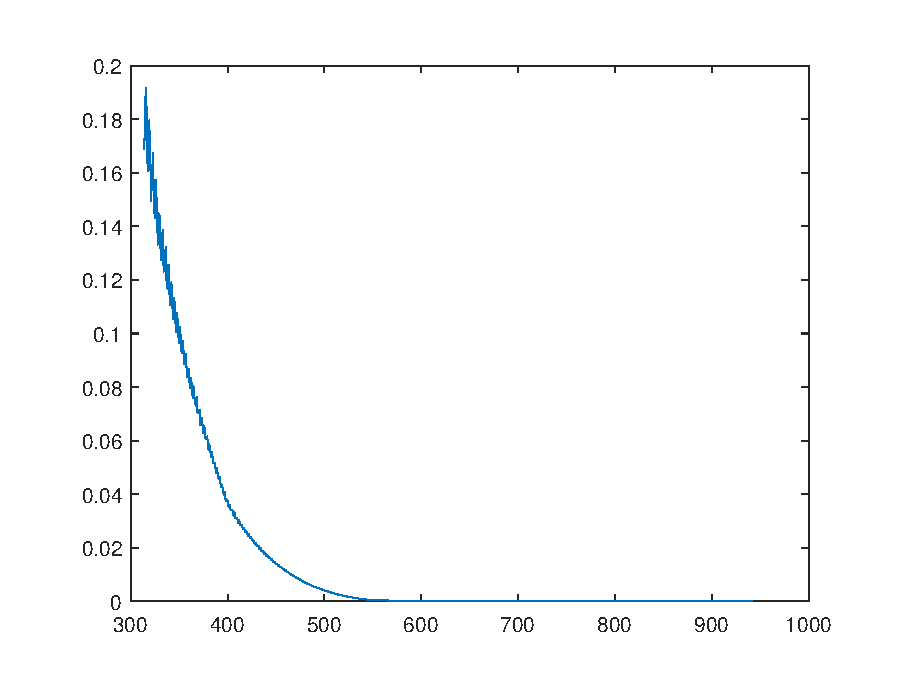
\includegraphics[width=0.4\textwidth]{exp8_1_1}}
	\subfigure{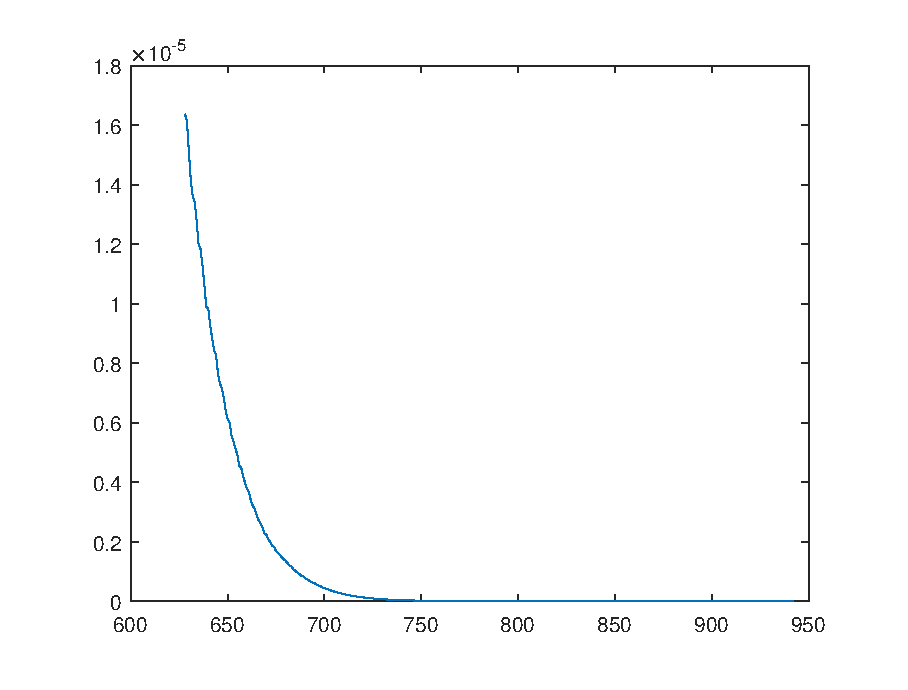
\includegraphics[width=0.4\textwidth]{exp8_1_2}}
\end{figure}

感觉CG方法的收敛性还是很不错的, 是远好于最速下降法的。
\subsection{第二问}
$n=200,400,600,800$, $tol=10^{-12}$时, 分别做出迭代次数和时间的折线图
\begin{figure}[h]
	\centering
	\subfigure{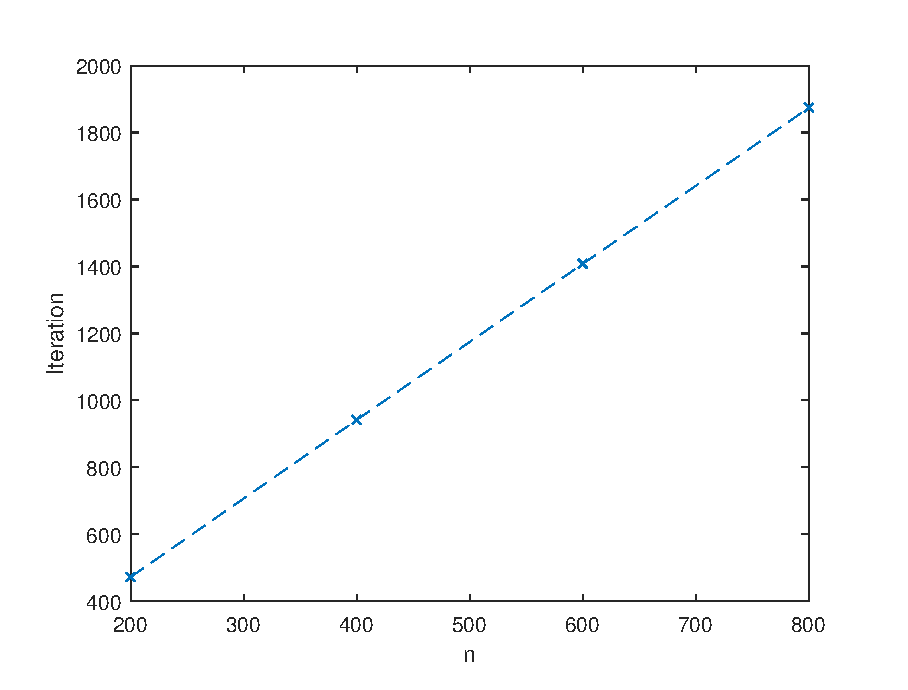
\includegraphics[width=0.4\textwidth]{exp8_1_3}}
	\subfigure{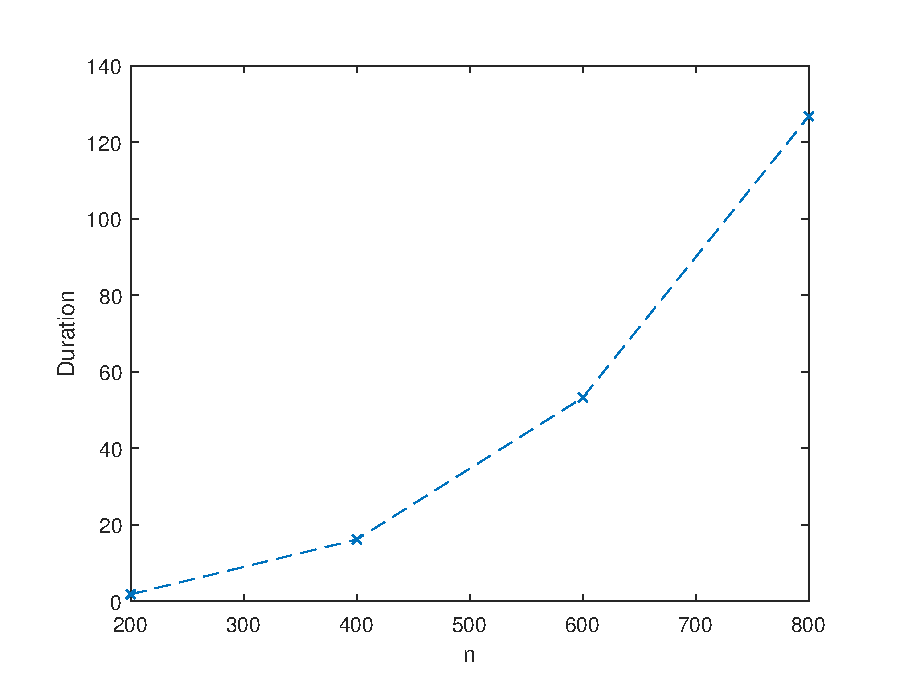
\includegraphics[width=0.4\textwidth]{exp8_1_4}}
\end{figure}
\section{实验12.1 Newton-Cotes公式求积分}
在教材\cite{1}中, 设$x_i=a+ih, h=\displaystyle\frac{b-a}{n}$, 作$f(x)$的n次Lagrange插值多项式$L_n(x)$, 令$x=a+th, t\in[0,n]$, 则$L_n(x)$可表示为
\begin{displaymath}
	L_n(x)=\sum_{i=0}^{n}(\prod_{j=0,j\neq i}^{n}\displaystyle\frac{x-x_j}{x_i-x_j})
\end{displaymath}

从而
\begin{displaymath}
	\int_{a}^{b}f(x){\rm d}x\approx\int_{a}^{b}L_n(x){\rm d}x=(b-a)\sum_{i=0}^{n}\displaystyle\frac{(-1)^{n-i}}{ni!(n-i)!}(\int_{0}^{n}\prod_{j=0,j\neq i}^n(t-j)f(x_i))=\sum_{i=0}^n\omega_if(x_i)
\end{displaymath}

即
\begin{displaymath}
	\omega_i=(b-a)\displaystyle\frac{(-1)^{n-i}}{ni!(n-i)!}=(b-a)C_i^{(n)}
\end{displaymath}

$\omega_i$ 被称为Cotes系数, 先给出编写的Newton-Cotes公式的系数及计算结果的函数
\begin{lstlisting}
	function [y,Ck]=NC(f,a,b,n)
	syms x
	Ck=zeros(1,n+1);
	h=(b-a)/n;
	x0=a:h:b;
	for i=1:n+1
		k=i-1;
		Ck(i)=(b-a)*(-1)^(n-k)/(n*factorial(k)*factorial(n-k));
		g=1;
		for j=[0:k-1,k+1:n]
			g=g*(x-j);
		end
		Ck(i)=Ck(i)*int(g,0,n);
	end
	y=Ck*subs(f,x,x0)';
	end
\end{lstlisting}

然后用以下代码调用, 绘制函数值的图像以及误差的图像得
\begin{lstlisting}
	clear
	clc
	syms x
	f=1/sqrt(1+x^2);
	y=zeros(1,50);
	for n=1:50
		tic
		[y(n),Ck]=NC(f,-5,5,n);
		toc
	end
	plot(1:50,y,'^-','MarkerEdgeColor','k','MarkerFaceColor','r','MarkerSize',3)
	R=abs(2*atan(5)-y);
	plot(1:50,R,'^-','MarkerEdgeColor','k','MarkerFaceColor','r','MarkerSize',3)
	h=legend('\(R=|\hat{y}-2\arctan x|\)');
	set(h,'Interpreter','latex')
\end{lstlisting}
\begin{figure}[h]
	\centering
	\subfigure[函数值图像]{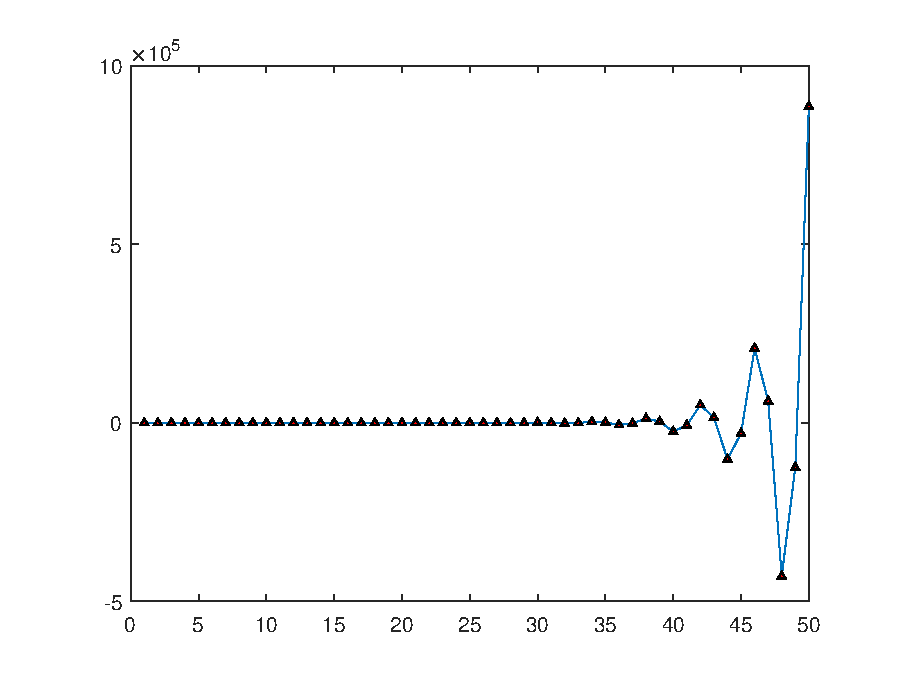
\includegraphics[width=0.4\textwidth]{exp12_1_1}}
	\subfigure[误差图像]{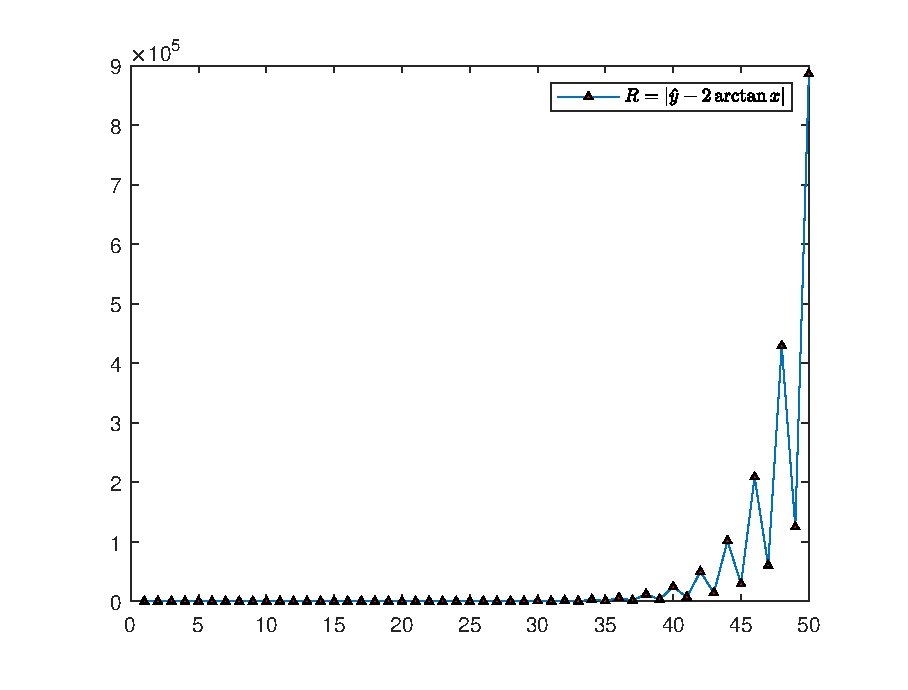
\includegraphics[width=0.4\textwidth]{exp12_1_2}}
\end{figure}

我们发现, 在$n$很大的时候, 误差是突增的, 这是因为Newton-Cotes系数在$n\geqslant 8$时不恒为正, 不能保证公式收敛到原积分。
\section{实验12.2 复合公式与高斯公式求积分}
\subsection{第一问}
首先给出Simpson公式的函数
\begin{lstlisting}
function y=SRule(f,a,b,n)
syms x
h=(b-a)/n;
num=subs(f,x,a:h/2:b);
tot=0;
for i=1:2:2*n-1
	tot=tot+num(i)/6+2*num(i+1)/3+num(i+2)/6;
end
y=tot*h;
end
\end{lstlisting}
\subsection{第二问}
先确定Gauss-Legendre公式的系数, 由书上的定理知, $n+1$次正交多项式的零点由下列对称三对角矩阵的特征值确定
\begin{displaymath}
	A=
	\begin{pmatrix}
		a_0 & \sqrt{b_1} & & & \\
		\sqrt{b_1} & a_1 & \sqrt{b_2} & & \\
		& \sqrt{b_2} & a_2 & \ddots & \\
		& & \ddots & \ddots & \sqrt{b_n}\\
		& & & \sqrt{b_n} & a_n
	\end{pmatrix}
\end{displaymath}

其中, $a_j=\displaystyle\frac{\beta_j}{\alpha_j}, b_j=\displaystyle\frac{\gamma_j}{\alpha_{j-1}\alpha_j}$, 参数${\alpha_j,\beta_j,\gamma_j}$是正交多项式$Q_{k+1}(x)$的三项递推公式
\begin{displaymath}
	Q_{j+1}(x)=(\alpha_jx-\beta_j)Q_j(x)-\gamma_jQ_{j-1}(x)
\end{displaymath}

对于Legendre多项式$\alpha_j=\displaystyle\frac{2n+1}{n+1}$, $\beta_j=0$, $\gamma_j=\displaystyle\frac{n}{n+1}$, 即
\begin{displaymath}
	a_j=0\qquad
	b_j=\displaystyle\frac{n^2}{(2n+1)(2n-1)}
\end{displaymath}

于是我们有下面的矩阵参数生成函数
\begin{lstlisting}
	function [a,b]=coefLegendre(n)
	% figure out the coefficient of nth symmetric matrix of Legendre
	a=zeros(n,1);
	b=a;
	b(1)=2;
	k=2:n;
	b(k)=1./(4-1./(k-1).^2);
	end
\end{lstlisting}

以及下面的系数生成函数
\begin{lstlisting}
function [x,w]=GL(n)
[a,b]=coefLegendre(n);
M=diag(a)+diag(sqrt(b(2:n)),1)+diag(sqrt(b(2:n)),-1);
[w,x]=eig(M);
x=diag(x);
w=w(1,:)'.^2*2;
[x,ind]=sort(x);
w=w(ind);
end
\end{lstlisting}

第一问第二问在同一个程序里操作, 代码为
\begin{lstlisting}
clear
clc
syms x
a=0;
b=1;
f=4*1/(1+x^2);
y=zeros(1,100);
n0=10000;
% Simpson
for n=1:100
	y(n)=SRule(f,a,b,n)-pi;
	if abs(y(n))<10^(-8) && n0==10000
		n0=n;
		y0=y(n);
	end
end
fprintf('n=%d, y=%f\n',n0,y0+pi)
plot(90:100,abs(y(90:100)),'^-','MarkerEdgeColor','k','MarkerFaceColor','r','MarkerSize',3)
hold on

% Gauss-Legendre
y=zeros(1,100);
n0=10000;
for n=1:100
	[x1,w]=GL(n);
	y(n)=(b-a)*0.5*subs(f,x,(ones(n,1)*(a+b)/2+(b-a)*x1/2)')*w-pi;
	if abs(y(n))<10^(-8) && n0==10000
		n0=n;
		y0=y(n);
	end
end
fprintf('n=%d, y=%f\n',n0,y0+pi)
plot(90:100,abs(y(90:100)),'^-','MarkerEdgeColor','k','MarkerFaceColor','r','MarkerSize',3)
legend('Simpson','Gauss-Legendre')
\end{lstlisting}

发现他们都是在$n=7$时达到精度, 此时$\hat{y}=3.141593$, 作出他们的残差图, 可以得到
\begin{figure}[h]
	\centering
	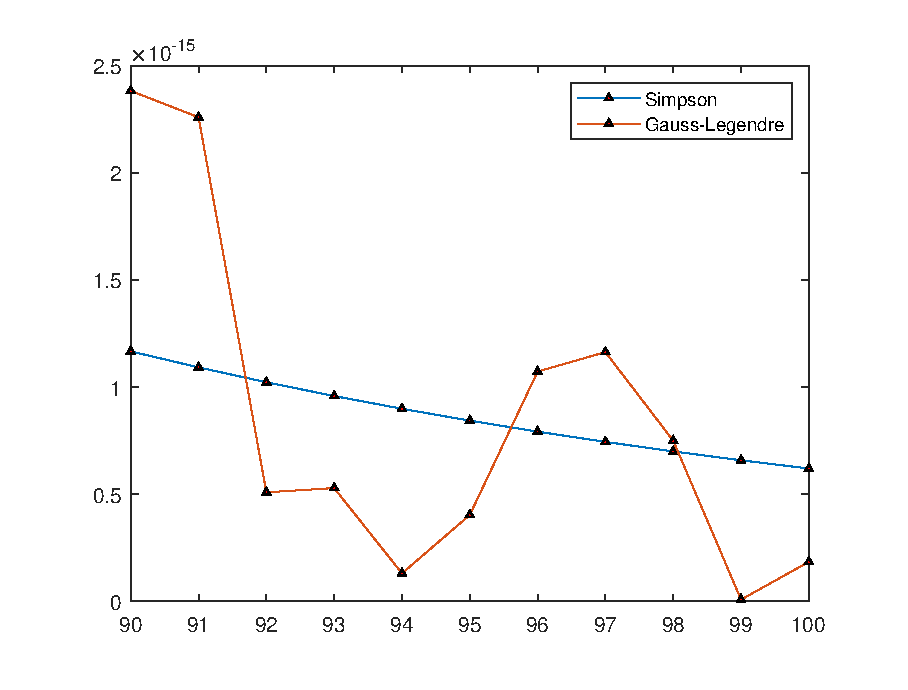
\includegraphics[width=0.75\textwidth]{exp12_2_1}
\end{figure}

发现他们的收敛速度是差不多的, 这是因为插值型求积公式的代数精度不超过$2n+1$, 而这里他们的代数精度都是$2n+1$
\section{实验12.3 数值积分公式的收敛性}
运行以下代码
\begin{lstlisting}
clear
clc
a=0;
b=1;
syms x alpha
f=abs(x)^(alpha+0.6);
% y1: apply T Rule
y1=zeros(5,200); % error
e1=zeros(5,200); % e1(i,t): e1(i,t) is the 1st n less than 10^-t when alpha=i-1
p1=1;
% y2: apply Simpson Rule
e2=e1;
p2=1;
y2=y1;
tru=zeros(1,5);
for i=0:4
	g=subs(f,alpha,i);
	tru(i+1)=int(g,x,a,b);
	for n=1:200
		y1(i+1,n)=TRule(g,a,b,n);
		y2(i+1,n)=SRule(g,a,b,n);
		e1(i+1,n)=abs(log(abs(y1(i+1,n)-tru(i+1))));
		e2(i+1,n)=abs(log(abs(y2(i+1,n)-tru(i+1))));
	end
end
figure(1)
plot(1:200,e1(1,:),1:200,e2(1,:))
legend('TRule','SRule')
title('$\alpha=0$','Interpreter','latex')
figure(2)
plot(1:200,e1(2,:),1:200,e2(2,:))
legend('TRule','SRule')
title('$\alpha=1$','Interpreter','latex')
figure(3)
plot(1:200,e1(3,:),1:200,e2(3,:))
legend('TRule','SRule')
title('$\alpha=2$','Interpreter','latex')
figure(4)
plot(1:200,e1(4,:),1:200,e2(4,:))
legend('TRule','SRule')
title('$\alpha=3$','Interpreter','latex')
figure(5)
plot(1:200,e1(5,:),1:200,e2(5,:))
legend('TRule','SRule')
title('$\alpha=4$','Interpreter','latex')
\end{lstlisting}

考虑到这是复合的梯形公式和Simpson公式, 因此这里不存在有震荡的现象, 也就是说不会有发散的现象出现, 我做了如下的可视化, 为了看的更清楚, 我们这里横坐标取复合公式的节点数$n+1$, 纵坐标是绝对误差的对数值的绝对值, 即
\begin{gather}
	y_1=|\ln (h\sum_{i=0}^{n-1}(\frac{f(x_i)}{6}+\frac{2f(x_{i+1/2})}{3}+\frac{f(x_{i+1})}{6})-\int_{0}^{1}|x|^{\alpha+3/5}{\rm d}x)|\nonumber\\
	y_2=|\ln (h\sum_{i=0}^{n-1}(\frac{f(x_i)}{2}+\frac{f(x_{i+1})}{2})-\int_{0}^{1}|x|^{\alpha+3/5}{\rm d}x)|\nonumber
\end{gather}

其中(1)式是复合Simpson公式的误差, (2)是复合梯形公式的误差
\begin{figure}[h]
	\centering
	\subfigure{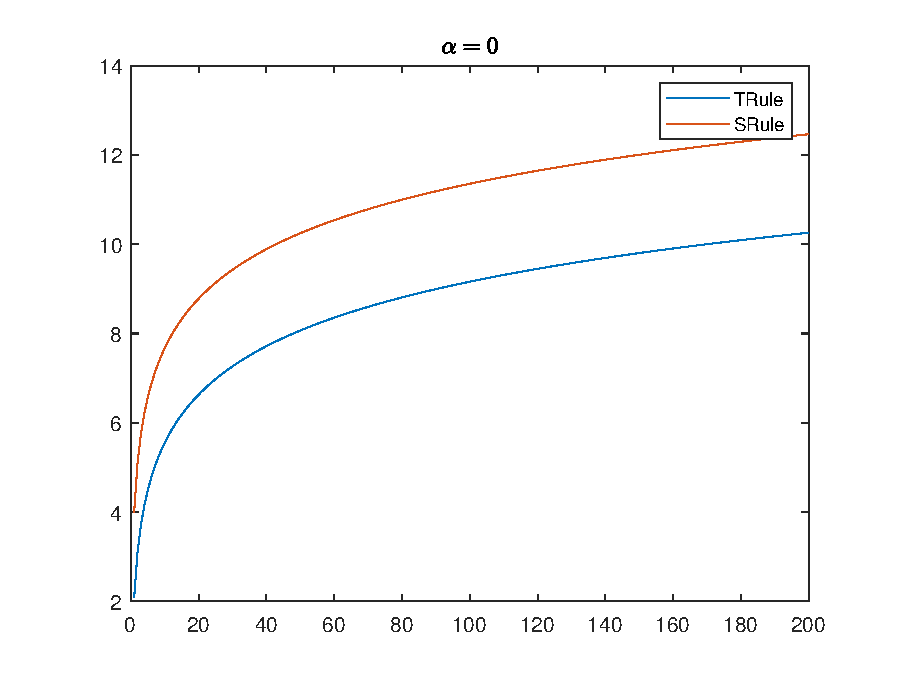
\includegraphics[width=0.4\textwidth]{exp12_3_0}}
	\subfigure{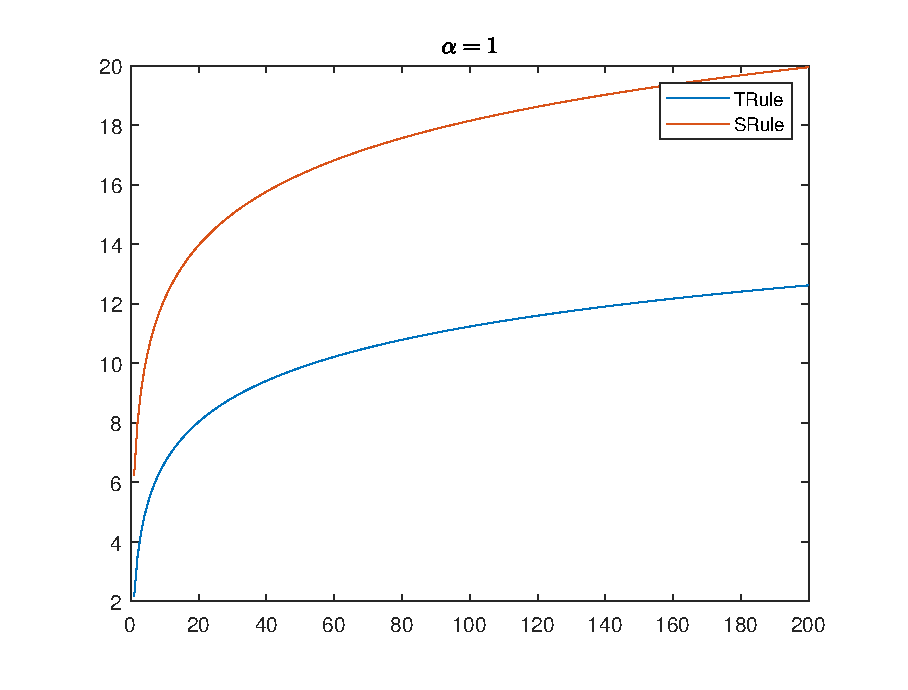
\includegraphics[width=0.4\textwidth]{exp12_3_1}}
	\subfigure{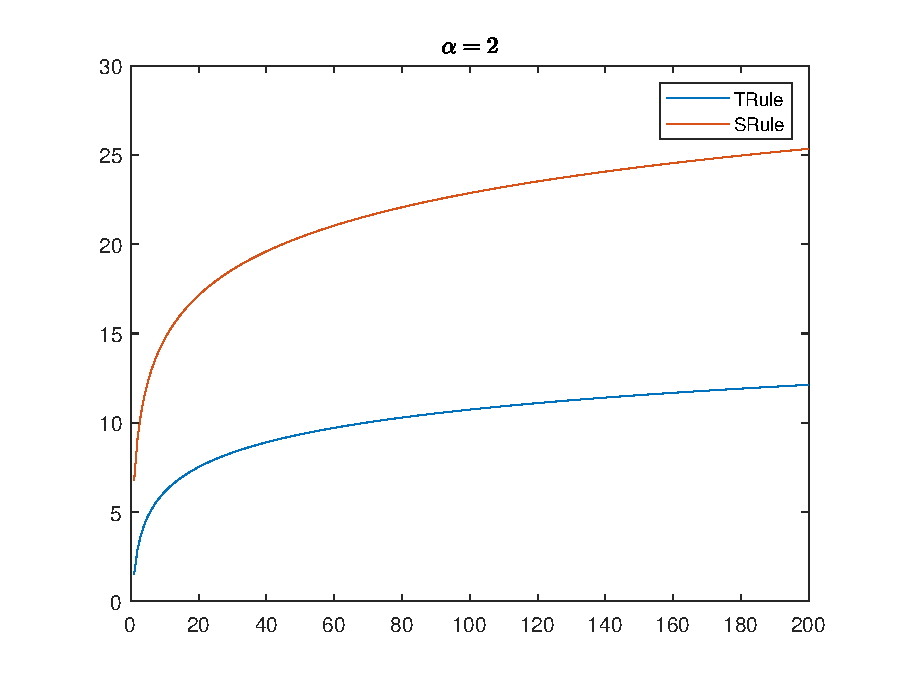
\includegraphics[width=0.4\textwidth]{exp12_3_2}}
	\subfigure{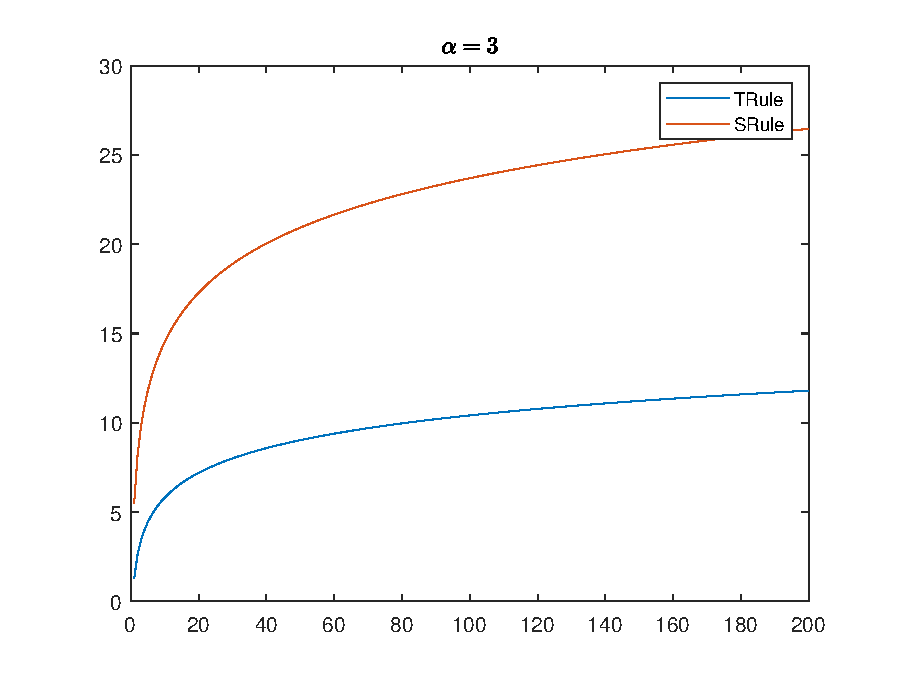
\includegraphics[width=0.4\textwidth]{exp12_3_3}}
	\subfigure{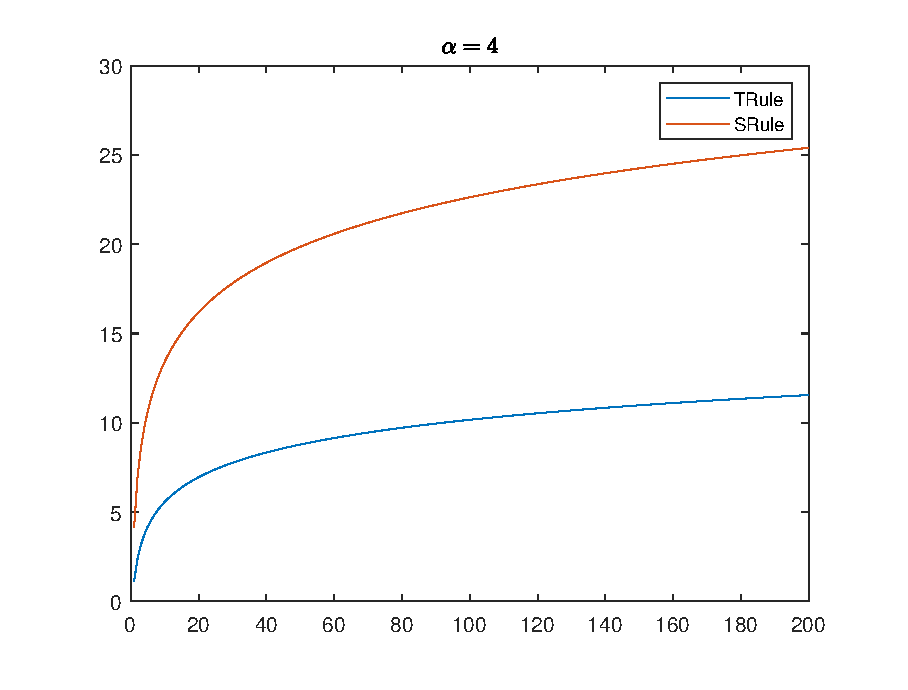
\includegraphics[width=0.4\textwidth]{exp12_3_4}}
\end{figure}

我们发现, 复合Simpson公式比复合梯形公式要收敛得快, 而且至少快了一倍。
%------------------------------------------------
% 感谢啥的乱七八糟的东西
%\phantomsection
%\section*{附录}
%\addcontentsline{toc}{section}{附录}


%----------------------------------------------------------------------------------------
%	REFERENCE LIST
%----------------------------------------------------------------------------------------
\phantomsection
\begin{thebibliography}{}
	\bibliographystyle{unsrt}
	\bibitem{1} 同济大学计算数学教研室. 现代数值计算[M]. 人民邮电出版社: 2014.9
\end{thebibliography}
%----------------------------------------------------------------------------------------

\end{document}